\begin{graphicspathcontext}{{./chapters/mas/architectures/imgs/},{./chapters/mas/architectures/imgs/auto/},{./chapters/mas/imgs/auto/},\old}

\begin{frame}{What is a State of an Agent?}
	\smaller
	\begin{definitionblock}{State}
	\emph{Description of the status} of a system that is waiting to execute a transition.
	\end{definitionblock}
	\begin{example}[State]
		\begin{description}
			\item[In an object $o$] \emph{named} set of values of all the fields of $o$, including the fields in the super classes
			\item[In an agent $a$] \emph{named} union of fields' values and states of data structures within the agent 
		\end{description}
	\end{example}
	\begin{definitionblock}{Transition}
	Set of actions to be executed when a condition is fulfilled or when an event is received. 
	\end{definitionblock}
	\begin{definitionblock}{Action}
	Description of changes of fields' values that cause a state change. 
\end{definitionblock}
\end{frame}

\begin{frame}{What is a Finite State Machine?}
	\begin{definitionblock}{Finite State Machine (FSM)}
		\begin{itemize}
		\item Mathematical model of computation in which the machine can be in exactly one of a finite number of states at any given time
		\item FSM can change from one state to another in response to some inputs
		\item $FSM = \langle S, s_0, T \rangle$ \\
			$S$: finite set of all the reachable states \\
			$s_0$: initial state of the machine \\
			$T : S \rightarrow S$, finite set of transitions 
		\end{itemize}
	\end{definitionblock}
\end{frame}

\figureslide[width=.6\linewidth]{Example of the Cleaning Robot}{fsm_cleaner}

\begin{frame}{FSM for Agents}
	\includeanimatedfigure[width=\linewidth]{fsm_foragent}
\end{frame}

\begin{frame}[fragile]{{Pseudo-Code:} State and Transition}
	\begin{sarllisting}[basicstyle=\scriptsize]
interface State {
	def getInActions : List<Action>
	def getEnterActions : List<Action>
	def getExitActions : List<Action>
	def getTransitions : List<Transition>
}

interface Transition {
	def isTriggered : boolean
	def getTargetState : State
	def getActions : List<Action>
}
	\end{sarllisting}
\end{frame}

\begin{frame}[fragile]{{Pseudo-Code:} State Machine}
\begin{sarllisting}[basicstyle=\scriptsize]
class StateMachine {
	// Holds a list of states for the machine
	var states : List<State>
	// Holds the initial state
	var initialState : State
	// Holds the current state
	var currentState = initialState

	// Checks and applies transitions
	def update : List<Action> {
		// Assume no transition is triggered by default
		var triggeredTransition : Transition = null
		// Search for the first transition that triggers
		val iterator = currentState.transitions.iterator
		while (iterator.hasNext && triggeredTransition === null) {
			val transition = iterator.next
			if (transition.isTriggered) {
				triggeredTransition = transition
			}
		}
\end{sarllisting}
\end{frame}

\begin{frame}[fragile]{{Pseudo-Code:} State Machine \insertcontinuationtext}
\begin{sarllisting}[basicstyle=\scriptsize]
		// Check if we have a transition to fire
		if (triggeredTransition !== null) {
			// Find the target state
			var targetState = triggeredTransition.targetState

			var actions = currentState.exitActions.clone
			actions += triggeredTransition.actions
			actions += targetState.entryActions

			currentState = targetState

			return actions
		} else {
			// Just return the current state's actions
			return currentState.inActions
		}
	}
}
\end{sarllisting}
\end{frame}

\begin{frame}{Performance Analysis}
	\begin{itemize}
		\item $O\left(n\times(1+m)\right)$ in memory
		\item $O(m)$ in time
		\item Where:
			\begin{itemize}
				\item $n$ is the number of states
				\item $m$ is the number of transitions per state
				\item Actions' list building is negligible
			\end{itemize}
		\vspace{1cm}
		\item Possible expensive functions:
			\begin{itemize}
				\item \code{State.getTransitions}
				\item \code{State.getTargetState}
			\end{itemize}
	\end{itemize}
\end{frame}

\begin{frame}{FSM in the Agent Lifecycle}
	\begin{center}
		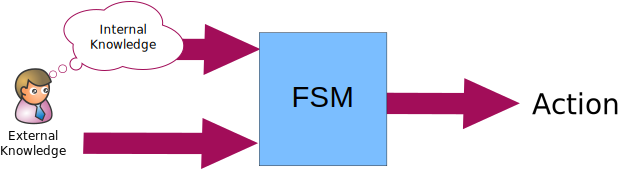
\includegraphics[width=.8\linewidth]{fsm_inagent}
	\end{center}
	\begin{columns}
		\begin{column}{.5\linewidth}
			\begin{block}{Current state is compatible with agent's State-of-Mind}
				\code{currentState == determineState(knowledge)}
				\begin{itemize}
					\item Use of the FSM
				\end{itemize}
			\end{block}
		\end{column}
		\begin{column}{.5\linewidth}
			\begin{alertblock}{Current state is incompatible with agent's State-of-Mind}
				\code{currentState != determineState(knowledge)}
				\begin{itemize}
					\item Force FSM current state?
					\item Continue with FSM current state?
				\end{itemize}
			\end{alertblock}
		\end{column}
	\end{columns}
\end{frame}

\begin{frame}[t,fragile]{Hard-Coded FSM}
	\begin{itemize}
	\item Few years back, almost all state machines were hard-coded
	\item Rules for transitions and execution of actions were part of the simulator code itself
	\vspace{.25cm}
	\item[$\oplus$] Very efficient implementation
	\item[$\ominus$] Static definition of the states and the transitions
	\end{itemize}
	\vspace{-.5cm}
	\begin{columns}
		\begin{column}[t]{.5\linewidth}
			\begin{sarllisting}[basicstyle=\tiny]
enum State {
	PATROL, DEFEND, SLEEP
}

class PatrollerFSM {
	var currentState = State::SLEEP
	
	def update(k : Knowledge)
			: List<Action> {
		switch(currentState) {
			case PATROL: {
				if (k.seePlayer) {
					currentState = DEFEND
					return #[]
				} else if (k.tired) {
					currentState = SLEEP
					return #[]
				} else {
			\end{sarllisting}
		\end{column}
		\begin{column}[t]{.5\linewidth}
			\begin{sarllisting}[basicstyle=\tiny]
					return #[RANDOM_MOVE]
				}
			}
			case DEFEND: {
				if (!k.seePlayer) {
					currentState = PATROL
					return #[]
				} else {
					return #[FIRE_GUN]
				}
			}
			case SLEEP: {
				if (!k.tired) {
					currentState = PATROL
				}
				return #[]
			}
		}
	}
}
\end{sarllisting}
		\end{column}
	\end{columns}
\end{frame}

\begin{frame}{Complex or Alternate Behaviors}
	\alertbox{How to express alternate behaviors with a FSM?}
	\begin{example}[Cleaning Robot]
		\begin{center}
			\includegraphics[width=.5\linewidth]{fsm_cleaner}
		\end{center}
	\end{example}
	\alertbox*{How introducing power down feature for the robot?}
\end{frame}

\figureslide{{Bad Answer:} cannot resume alternate state}{fsm_cleaner_bad0}

\figureslide{{Bad Answer:} duplication of states}{fsm_cleaner_bad1}

\figureslide{{Good Answer:} hierarchical state machine}{fsm_cleaner_good}

\begin{frame}[t,fragile]{{Pseudo-Code:} Abstract HFSM}
\begin{sarllisting}[basicstyle=\scriptsize]
class UpdateResult {
	var actions : List<Action>
	var transitions : List<Transition>
	var level : int
}

abstract class AbstractHFSM {

	def getActions : List<Action> {
		#[]
	}

	def update : UpdateResult {
		new UpdateResult => [
			actions = getActions
			transition = null
			level = 0
		]
	}

	abstract def getStates : List<AbstractHFSM>
}
\end{sarllisting}
\end{frame}

\begin{frame}[fragile]{{Pseudo-Code:} State and Transition}
	\begin{columns}
		\begin{column}{.5\linewidth}
			\begin{sarllisting}[basicstyle=\scriptsize]
class State extends AbstractHFSM { 
	def getStates {
		// If we're just a state
		// then the stack is just us
		#[ this ]
	}

	// As in the standard FSM
	// implementation...
	def getActions {...}
	def getEnterActions {...}
	def getExitActions {...}
	def getTransitions {...}
}
			\end{sarllisting}
		\end{column}
		\begin{column}{.5\linewidth}
			\begin{sarllisting}[basicstyle=\scriptsize]
class Transition {
	// Returns the different in
	// levels of the hierarchy
	// from the source to the target
	// of the transition
	def getLevel : int {...}

	// As in the standard FSM implementation...
	def isTriggered {...}
	def getTargetState {...}
	def getActions {...}
}
			\end{sarllisting}
		\end{column}
	\end{columns}
\end{frame}

\begin{frame}[t,fragile]{{Pseudo-Code:} HFSM}
	\begin{sarllisting}[basicstyle=\scriptsize]
class HierarchicalFiniteStateMachine extends AbstractHFSM {
	// List of states at this level of the hierarchy
	var states : List<State>

	// The initial state for when the machine has to current state
	var initialState : State

	// The current state of the machine
	var currentState = initialState

	// Gets the current state stack
	def getStates : List<AbstractHFSM>
		this.currentState?.getStates
	}
	\end{sarllisting}
\end{frame}

\begin{frame}[t,fragile]{{Pseudo-Code:} HFSM \insertcontinuationtext}
	\begin{sarllisting}[basicstyle=\scriptsize]
	// Recursively updates the machine
	def update : UpdateResult {
		// If we're in no state, use the initial state
		if (currentState === null) {
			currentState = initialState
			return currentState.getEntryActions
		}

		// Try to find a transition in the current state
		var triggeredTransition = null
		val iterator = currentState.transitions.iterator
		while (iterator.hasNext &&
				triggeredTransition === null) {
			val transition = iterator.next
			if (transition.isTriggered)
				triggeredTransition = transition
		}
	\end{sarllisting}
\end{frame}

\begin{frame}[t,fragile]{{Pseudo-Code:} HFSM \insertcontinuationtext}
	\vspace{-.25cm}
	\begin{sarllisting}[basicstyle=\scriptsize]
		// If we're found one, make a result structure for
		// it
		var result = UpdateResult
		if (triggeredTransition !== null) {
			result = new UpdateResult => [
				actions = #[]
				transition = triggeredTransition
				level = triggeredTransition.level
			]
		} else {
			// Otherwise recurse down for a result
			result = currentstate.updaTransitionte
		}

		// Check if the result contains a transition
		if (result.transition !== null) {
			// Act based on its level
			if (result.level === 0) {
				// Its on our level: honor it
				targetState = result.transition.targetState
				result.actions += currentState.exitActions
				result.actions += result.transition.actions
				result.actions += targetState.enterActions
	\end{sarllisting}
\end{frame}

\begin{frame}[t,fragile]{{Pseudo-Code:} HFSM \insertcontinuationtext}
	\vspace{-.25cm}
	\begin{sarllisting}[basicstyle=\scriptsize]
				// Set our current state
				currentState = targetState
				// Add our normal action (we may be a state)
				result.actions += getActions
				
				// Clear the transition, so nobody else does it
				result.transition = null
			} else if (result.level > 0) {
				// Its destined for a higher level
				// Exit our current state
				result.actions += currentState.exitActions
				currentState = null
				// Decrease the number of levels to go
				result.level --
			} else {
				// It needs to be passed down
				targetState = result.transition.targetState
				targetMachine = targetState.parent
				result.actions += result.transition.actions
				result.actions += targetMachine.updateDown(
				targetState, -result.level)
				// Clear the transition, so nobody else does it
				result.transition = null
			}
	\end{sarllisting}
\end{frame}

\begin{frame}[t,fragile]{{Pseudo-Code:} HFSM \insertcontinuationtext}
	\begin{sarllisting}[basicstyle=\scriptsize]
		} else {
			// We can simply do our normal action
			result.actions += getActions
		}

		// Return the accumulated result
		return result
	}

	// Recurses up the parent hierarchy, transitioning
	// into each state in turn for the given number of
	// levels
	def updateDown(state : AbstractHFSM, level : int) {
		// if we're at top elvel, continue recursing
		if (level > 0) {
			// Pass ourself as the transition state to our parent
			actions = parent.updateDown(this,level - 1)
		} else {
			// Otherwise we have no action to add to
			actions = #[]
		}
	\end{sarllisting}
\end{frame}

\begin{frame}[t,fragile]{{Pseudo-Code:} HFSM \insertcontinuationtext}
	\begin{sarllisting}[basicstyle=\scriptsize]
		// If we have a current state, exit it
		if (currentState !== null)
			actions += currentState.exitActions

		// Move to the new state, and return all the actions
		currentState = state
		actions += state.getEnterActions
		return actions
	}
}
	\end{sarllisting}
\end{frame}

\begin{frame}[t,fragile]{{Pseudo-Code:} Sub-machine}
	\begin{sarllisting}[basicstyle=\scriptsize]
class SubMachineState
		extends State, HierarchicalStateMachine

	// Route get action to the state
	def getActions {
		State::getActions
	}

	// Route update to the state machine
	def update {
		HierarchicalFiniteStateMachine.update
	}

	// We get states by adding ourself to our active children
	def getStates {
		if (currentState !== null)
			return #[this] + currentState.states
		else
			return #[this]
	}
}
	\end{sarllisting}
\end{frame}

\begin{frame}[t]{Combining Decision Trees and State Machines}
	\begin{itemize}
	\item Decision trees are an efficient way of matching series of conditions
	\item Decision trees and FSM could be combined by replacing transitions in a FSM by a decision tree.
	\end{itemize}
	\begin{center}
		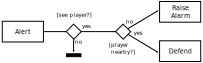
\includegraphics[width=.8\linewidth]{fsm_dt}
	\end{center}
	\alertbox{Is it different than a composed boolean condition? \\
	$\Rightarrow$ it may be optimization for avoiding evaluation of the same boolean sub-expressions \\
	$\Rightarrow$ dynamic building of the transition}
\end{frame}

\end{graphicspathcontext}

\endinput
